\documentclass[xcolor=dvipsnames]{beamer}
\usecolortheme[named=OliveGreen]{structure}
\usetheme[height=7mm]{Rochester}
\usepackage{graphicx}
\usepackage{subfigure}
\usepackage{tikz}
\usetikzlibrary{arrows,backgrounds,fit,petri,positioning,shapes}

\setbeamertemplate{items}[ball]
\setbeamertemplate{blocks}[rounded][shadow=true]
\setbeamercovered{invisible}
\setbeamertemplate{navigation symbols}{} % Remove navigation symbols
\setbeamertemplate{headline}{}
\setlength{\parskip}{1em}

\newcommand{\reals}{\mathbb{R}}
\newcommand{\trans}{\mathrm{T}}

\DeclareMathOperator{\Tr}{Tr}
\DeclareMathOperator*{\argmax}{argmax}
\DeclareMathOperator*{\argmin}{argmin}
\DeclareMathOperator{\diag}{diag}
\DeclareMathOperator{\rank}{rank}
\newcommand{\Normal}[1][]{\mathcal{N}_{#1}}
\newcommand{\Wishart}[1][]{\mathcal{W}_{#1}}

\newcommand{\prob}{\mathbb{P}}
\newcommand{\E}{\mathbb{E}}
\DeclareMathOperator{\RSS}{RSS}

\newtheorem{proposition}[theorem]{Proposition}
\newtheorem{remark}[theorem]{Remark}


\title{Regularized Laplacian Estimation and \\ Fast Eigenvector Approximation}
\author{Patrick~O.~Perry \and Michael~W.~Mahoney}
\institute[NYU Stern and Stanford] {
  NYU Stern \and Stanford University
}
\date{\today}

\begin{document}
% For every picture that defines or uses external nodes, you'll have to
% apply the 'remember picture' style. To avoid some typing, we'll apply
% the style to all pictures.
\tikzstyle{every picture}+=[remember picture]

% By default all math in TikZ nodes are set in inline mode. Change this to
% displaystyle so that we don't get small fractions.
\everymath{\displaystyle}

\begin{frame}
  \titlepage
\end{frame}


\begin{frame}[c]
  \begin{block}{}
  \begin{center}
    \huge{Introduction}
  \end{center}
  \end{block}
\end{frame}


\begin{frame}
  \begin{block}{Eigenvectors reveal structure}
  \begin{description}
    \item[Modularity matrix] community detection
    \item[Graph Laplacian] spectral clustering
    \item[Covariance matrix] factor analysis
  \end{description}
  \end{block}
  
  One way to visualize and simplify high-dimensional data is to form a matrix
  capturing structural information about the dataset and then to focus on
  the leading eigenvectors of this matrix.
\end{frame}


\begin{frame}
  \begin{block}{Diffusions reveal structure}
  \begin{description}
    \item[Heat diffusion] evolution determined by heat equation
    \item[PageRank surfer] random walk with teleportation
    \item[Truncated random walk] finite-length random walk
  \end{description}
  \end{block}

  Alternatively, one can distributed random charge on the data points and
  let the distribution of the charge according to a diffusion; the properties
  of this diffusion are related to the geometry of the dataset.

  Mahoney~and~Orecchia~\cite{MO11-implementing} showed that diffusions arise
  as solutions to \emph{regularized} eigenvector problems.
\end{frame}


\begin{frame}
  \begin{block}{Regularization}
  \begin{description}
    \item[Original problem] minimize $f(x)$
    \item[Regularized problem] minimize $f(x) + \frac{1}{\eta} g(x)$
  \end{description}
  \end{block}

  Regularization is a general principle where we add a penalty function to
  the optimization criterion.  E.g., $g(x) = \|x\|_2$ or $g(x) = \|x\|_1$.
  The solution to the regularized problem is
  often less sensitive to perturbations of the input data, and thus is
  has better statistical robustness.
\end{frame}

\begin{frame}
\centering
{\Large Big picture}
\vspace{-4em}

\begin{tikzpicture}[scale=2]
    \matrix[nodes={draw, ultra thick, fill=blue!20, minimum width=6em, minimum height=4em},
        row sep=1em,column sep=3em,ampersand replacement=\&] {
      \node[ellipse] (graphs) {Graphs};\&
      \node[ellipse] (regularization) {Regularization};\&
      \node[ellipse] (structure) {$\stackrel{\hbox{Diffusion/}}{\hbox{Structure}}$};\\
    };
    \path[<->, ultra thick]
      (regularization)
        edge node[auto, rotate=45, anchor=south west] {Mahoney \& Orecchia}
          (structure)
      (graphs)
        edge [bend right=30] node[below] {Empirical experience}
          (structure);
    \path[<->, ultra thick, dashed]
      (graphs)
        edge node[above, rotate=45, anchor=south west] {This work}
          (regularization);
\end{tikzpicture}
From empirical experience, we know that certain diffusions are more
appropriate for certain classes of graphs.
From Mahoney and Orecchia, we know certain diffusions arise as solutions
to certain regularized eigenvector problems.
The current work attempts to complete the circle by showing that certain 
type of regularization make certain implicit assumptions about structural
properties of the graph.
\end{frame}


\begin{frame}[c]
  \begin{block}{}
  \begin{center}
    \huge{Background}
  \end{center}
  \end{block}
\end{frame}


\begin{frame}
  \begin{block}{Notation for a weighted undirected graph}
  \begin{itemize}
    \item vertex set $V = \{ 1, \dotsc, n \}$ 
    \item edge set $E \subset V \times V$
    \item edge weight function $w : E \to \mathbb{R}^+$
    \item degree function $d : V \to \mathbb{R}^+$, $d(u) = \sum_v w(u,v)$
    \item diagonal degree matrix $D \in \mathbb{R}^\times{V \times V}$, $D(v,v) = d(v)$
    \item combinatorial Laplacian $L_0 \in \mathbb{R}^{V \times V}$,
    	$L_0(u,v) = \begin{cases}
		-w(u,v) &\text{when $u \neq v$} \\
		d(u) - w(u,v) &\text{otherwise.}
	\end{cases}$
    \item normalized Laplacian $L = D^{-1/2} \, L_0 \, D^{-1/2}$
  \end{itemize}
  \end{block}
  We will need the above notation.
\end{frame}

\begin{frame}
  \begin{block}{Diffusion-based procedures}
  \begin{description}
    \item[Heat Kernel] Charge evolves according to the heat equation
    	$\frac{\partial H_t}{\partial t} = - L H_t$.
    \item[PageRank] Charge at a node evlolves by either moving to a neighbor
    	of the current node or teleporting to a random node.
    \item[Lazy Random Walk] Charge either stays at the current node or moves
        to a neighbor.
  \end{description}
  \end{block}
  In each of these diffusions, we distributed charge on the vertices of a
  graph, and let the charge evolve according to certain dynamics.  The
  specific choice of the dynamics (Heat Kernel, PageRank, or Lazy Random Walk)
  is determined by structural features of the graph.  To date, there is some
  empirical understanding of which dynamics are appropriate for which classes
  of graphs, but no theoretical basis for these differences.
\end{frame}

\begin{frame}
  \begin{block}{Original eigenvector problem}
  \begin{columns}
  \column{0.3\textwidth}
    \begin{equation*}
    \begin{aligned}
    & \underset{x}{\text{minimize}}
    & & x^\mathrm{T} L x \\
    & \text{subject to}
    & & \| x \|_2 = 1, \\
    & & & x^\mathrm{T} D^{1/2} 1 = 0 \\
    & & &
    \end{aligned}
    \end{equation*}
    (standard form)
  \column{0.3\textwidth}
    \begin{equation*}
    \begin{aligned}
    & \underset{X}{\text{minimize}}
    & & \mathrm{Tr}(L X)\\
    & \text{subject to}
    & & \mathrm{Tr}(X) = 1, \\
    & & & X D^{1/2} 1 = 0, \\
    & & & X \succeq 0
    \end{aligned}
    \end{equation*}
    (relaxed form)
  \end{columns}
  \end{block}
  The correspondence between the two is that the solutions satisfy
  $x x^\mathrm{T} = X$.
\end{frame}

\begin{frame}
  \begin{block}{Regularized eigenvector problem}
    \begin{equation*}
    \begin{aligned}
    & \underset{X}{\text{minimize}}
    & & \mathrm{Tr}(L X) + \tfrac{1}{\eta} G(X) \\
    & \text{subject to}
    & & \mathrm{Tr}(X) = 1, \\
    & & & X D^{1/2} 1 = 0 \\
    & & & X \succeq 0
    \end{aligned}
    \end{equation*}
  \end{block}
\end{frame}

\begin{frame}
  \begin{block}{Mahoney \& Orecchia's result}
    \centering
    \begin{tabular}{ccc}
      Penalty &\phantom{MMM} & Solution \\
      \hline
      $\mathrm{Tr}(X \log X) - \mathrm{Tr}(X)$ && Heat Kernel \\
      $- \log |X|$ && PageRank  \\
      $\mathrm{Tr}(X^k)$ && Lazy Random Walk
    \end{tabular}
  \end{block}
  Mahoney \& Orecchia's result shows that certain choices of the penalty
  function $G(X)$ result in the solutions of the regularized eigenvector
  problem involving certain diffusions (summarized by the table).
\end{frame}


\begin{frame}
  \begin{block}{}
  \begin{center}
    \huge{Statistical framework for regularized graph estimation}
  \end{center}
  \end{block}
\end{frame}

\begin{frame}
  \begin{block}{Analogy with regularized linear regression}
  \begin{itemize}
    \item Observe $n$ predictor-response pairs in $\mathbb{R}^p \times \mathbb{R}$:
      $(x_1, y_1), \dotsc, (x_n, y_n)$
    \item Original problem: find $\beta$ such that $\beta' x_i \approx y_i$; minimize $F(\beta) =
    \sum_i \|y_i - \beta' x_i \|_2^2$
    \item Regularized problem: minimize $F(\beta) + \lambda \| \beta \|_2^2$
    (ridge) or minimize $F(\beta) + \lambda \| \beta \|_1$ (lasso)
  \end{itemize}
  \end{block}
\end{frame}

\begin{frame}
  \begin{tikzpicture}
    [pre/.style={<-, >=stealth', semithick},
     post/.style={->, >=stealth', semithick},
     py/.style={color=blue},
     pbeta/.style={color=red},
     scale=0.75, transform shape]

    \node (model)
      {$y_i | x_i, \beta \sim \mathrm{Normal}(x_i' \beta, \sigma^2)$} ;
    \node (likelihood) [py, below=of model, yshift=1cm]
      {$\exp\{ -\frac{1}{2 \sigma^2} \sum_i (y_i - \beta' x_i)^2\}$};

    \node (normal)  [below left=of likelihood, xshift=2.5cm]
      {$\beta_j \sim \mathrm{Normal}(0, \tau^2)$};
    \node (normal prior) [pbeta, below=of normal, yshift=1cm]
      {$\exp\{ -\frac{1}{2 \tau^2} \|\beta\|_2^2 \}$};

    \node (laplace) [below right=of likelihood, xshift=-2.5cm]
      {$\beta_j \sim \mathrm{Laplace}(\mu)$};
    \node (laplace prior) [pbeta, below=of laplace, yshift=1cm]
      {$\exp\{ -\frac{1}{\mu} \|\beta\|_1 \}$};

    \node (tee) [circle, at= (model |- normal), yshift=1cm, inner sep=0,
                 fill=black, minimum size=0.5pt, draw] {}
      edge[pre] (likelihood)
      edge[post] (normal)
      edge[post] (laplace);

    \node (l2) [below=of normal prior]  {$\ell_2$-regularized LS}
      edge[pre] (normal prior);
    \node (l1) [below=of laplace prior] {$\ell_1$-regularized LS}
      edge[pre] (laplace prior);

    \node (prior label) [left=of normal]                    {Prior};
    \node (pbeta label) [pbeta, at=(prior label |- normal prior)]  {$p(\beta)$};
    \node (model label) [at=(prior label |- model)]         {Model};
    \node (py label)    [py, at=(prior label |- likelihood)]    {$p(y | \beta)$};
    \node (map label)   [at=(prior label |- l2), align=center] {MAP\\ Estimate};
  \end{tikzpicture}

  Regularization is equivalent to ``Bayesianization'' in the following sense:
  the solution to the regularized problem is equal to the maximim \textit{a posteriori} probability
  (MAP) estimate of the parameter with a prior determined by the
  regularization penalty.
\end{frame}

\begin{frame}
\begin{block}{Bayesian inference for the population Laplacian (broadly)}
  \begin{itemize}
    \item population Laplacian, $\mathcal{L}$ from prior $p(\mathcal{L})$
    \item observed (sample) Laplacian from distribution $p(L \mid \mathcal{L})$
    \item estimate $\mathcal{\hat L} = \argmax_{\mathcal{L}} \{ p(\mathcal{L} \mid L) \}$
    \item equivalently,
      $\mathcal{\hat L} = \argmin_{\mathcal{L}} \{ -\log p(L \mid \mathcal{L}) -\log p(\mathcal{L}) \}$
  \end{itemize}
\end{block}

  To apply the Bayesian formalism to the Laplacian eigenvector problem, we
assume that there exists a ``population'' Laplacian $\mathcal{L}$; we construe
the observed (sample) Laplacian as a noisy version of $\mathcal{L}$.  In
estimating $\mathcal{L}$, the negative log of the likelihood plays the role of
the optimization criterion; the negative log of the prior distribution for
$\mathcal{L}$ plays the role of the penalty function.

\end{frame}


\begin{frame}
\begin{block}{Bayesian inference for the population Laplacian (specifics)}
  \begin{itemize}
    \item two parameters, $m$ (scalar) and $U$ (function)
    \item assume $\mathcal{L} \in \mathcal{X}$, where
      \[
        \mathcal{X} = \{ X : X \succeq 0, \, X D^{1/2} 1 = 0, \, \rank(X) = n - 1 \}
      \]
    \item prior
      \(
        p(\mathcal{L}) \propto \exp\{ - U(\mathcal{L})\}
      \)
    \item model $L \sim \tfrac{1}{m} \mathrm{Wishart}(\mathcal{L}, m)$, i.e.
      \[
        p(L \mid \mathcal{L})
          \propto
            \frac{\exp\{-\frac{m}{2} \mathrm{Tr}(L \, \mathcal{L}^+)\}}
                 {|\mathcal{L}|^{m/2}} 
      \]
  \end{itemize}
\end{block}
\end{frame}


\begin{frame}[c]
  \begin{block}{}
  \begin{center}
    \huge{A prior related to the PageRank procedure}
  \end{center}
  \end{block}
\end{frame}


\begin{frame}
  \begin{block}{Prior density}
    Let $\mathcal{L}^{+} = \tau O \Lambda O'$ be the spectral decomposition of
    the pseudoinverse of the normalized Laplacian $\mathcal{L}$, where
    $\tau \geq 0$ is a scale factor, $O \in \mathbb{R}^{n \times n - 1}$ is
    an orthogonal matrix, and
    $\Lambda = \mathrm{diag}\big(\lambda(1), \dotsc, \lambda(n-1)\big)$,
    where $\sum_v \lambda(v) = 1$.  The prior takes the form:
    \[
      p(\mathcal{L}) \propto p(\tau) \prod_{v=1}^{n-1} \lambda(v)^{\alpha - 1}
    \]
    Note $\lambda$ is unordered.
  \end{block}
  This is the only prior for which $\lambda$ is exchangeable and neutral
  (Fabius, 1973).
\end{frame}


\begin{frame}
  \begin{proposition}
    If $\mathcal{\hat L}$ is the MAP estimate of $\mathcal{L}$, with
    $\hat \tau = \Tr(\mathcal{\hat L}^+)$ and
    $\hat \Theta = \hat \tau^{-1} \mathcal{\hat L}^+$,
    then $\hat \Theta$ solve
    the Mahoney-Orecchia regularized SDP with $G(X) = -\log |X|$ and
    $\eta$ defined by
    \[
      \eta = \frac{m \, \hat \tau}{m + 2\,(\alpha - 1)}.
    \]
  \end{proposition}
\end{frame}

\begin{frame}[c]
  \begin{block}{}
  \begin{center}
    \huge{Empirical evaluation}
  \end{center}
  \end{block}
\end{frame}

\begin{frame}
  \begin{center}
  \begin{tikzpicture}
    [vertex/.style={circle,draw=blue!50,fill=blue!20,thick},
     txt/.style={scale=5,transform shape},
     scale=0.2,transform shape]
    \foreach \x in {1,...,5} {
      \foreach \y in {1,...,6} {
        \draw (\x,\y) -- +(0,1);
	\draw (\x,\y) -- +(1,0);
	\node at (\x,\y) [vertex] {};
      }
      \draw (\x,7) -- +(1,0);
      \node at (\x,7) [vertex] {};
    }
    \foreach \y in {1,...,6} {
        \draw (6,\y) -- +(0,1);
	\node at (6,\y) [vertex] {};
    }
    \node at (6,7) [vertex]{};

    \node at (0,0) (l0 lower) {};
    \node at (7,8) (l0 upper) {};

    \node at (0,4)   (l0 h) [txt] {$h$};
    \node at (3.5,8) (l0 w) [txt] {$w$};

    \begin{scope}[yshift=-11cm]
      \begin{scope}[xshift=-4.5cm]
        \draw (1,1) rectangle (6,7);
        \draw (2,5) node[vertex] {} -- (3,5) node[vertex] {};
        \draw (5,3) node[vertex] {} -- (5,2) node[vertex] {};
        \node at (0,0) (s lower) {};
      \end{scope}

      \begin{scope}[xshift=4.5cm]
        \draw (1,1) rectangle (6,7);
        \draw (2,5) node[vertex] {} -- (5,2) node[vertex] {};
        \draw (5,3) node[vertex] {} -- (3,5) node[vertex] {};
        \node at (7,8) (s upper) {};
      \end{scope}

      \draw[->,thin,>=stealth'] (2,4) to [out=30,in=150] (5,4);

      \node[draw,rectangle,fit=(s lower)(s upper)] (swap) {};
      \node (swap text) [below=of swap, yshift=8mm] [txt] {$s$ swaps};
    \end{scope}

    \begin{scope}[yshift=-19cm]
      \node at (3.5,0) [scale=10, align=center, transform shape] (l) {$\mathcal{L}$};
    \end{scope}

    \node (r1) [fit=(l0 lower)(l0 upper)] {};
    \node (r2) [fit=(swap)(swap text)] {};
    \node (r3) [fit=(l)] {};

    \draw[->,ultra thick,>=latex] (r1) to (r2);
    \draw[->,ultra thick,>=latex] (r2) to (r3);

    \node [right=of r1, align=left] (l0 text) [txt]
      {
        $n = w \, h$ nodes, \\
        $\mu = 2 \, w \, h - w - h$ edges
      };
  \end{tikzpicture}
  \end{center}
  \vspace{-2em}

  We generate a population Laplacian $\mathcal{L}$ by performing $s$ edge
  swaps starting from a 2-dimensional grid with $n$ nodes and $\mu$ edges.
\end{frame}

\begin{frame}
  \centering
  \makebox{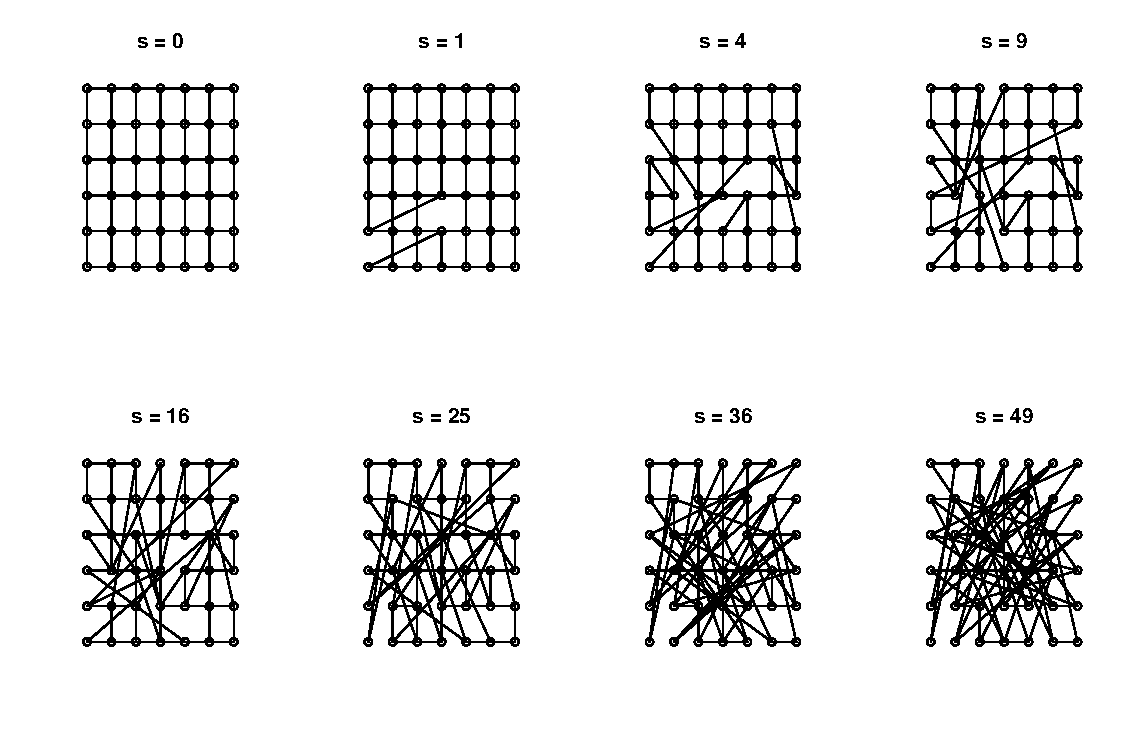
\includegraphics[scale=0.55]{plots/interpolate-graphs}}
  When $s = 0$ the population graph with Laplacian $\mathcal{L}$ is
  low-dimensional; as $s \to \infty$, the graph becomes an expander.
\end{frame}


\begin{frame}
\begin{figure}[h]
    \centering
    \subfigure[Eigenvalues of $\Theta = (\Tr(\mathcal{L^+}))^{-1} \mathcal{L^+}$]{
      \makebox{\label{F:interpolate}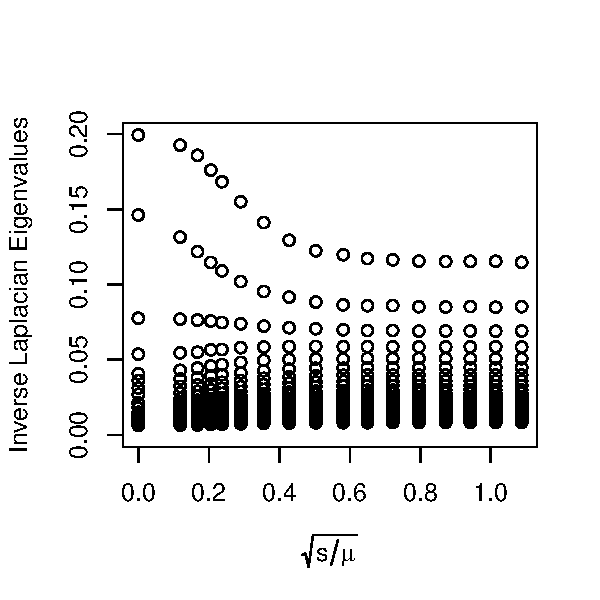
\includegraphics[scale=0.5]{plots/interpolate}}
    }
    \subfigure[Draws from Dirichlet($\alpha$)]{
      \makebox{\label{F:dirichlet}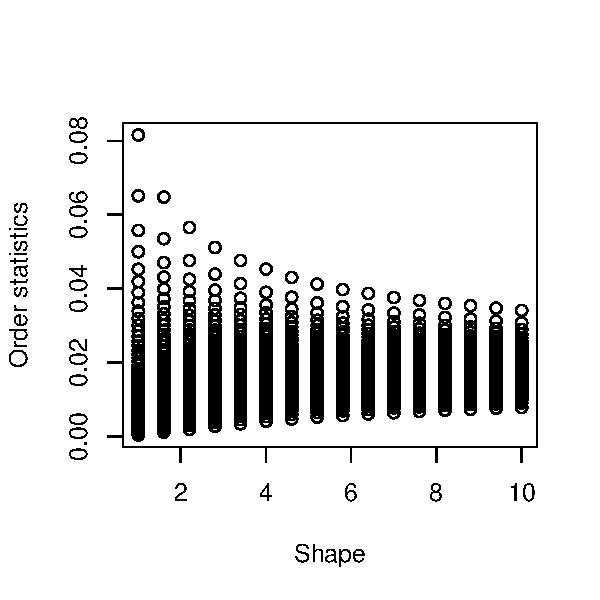
\includegraphics[scale=0.5]{plots/dirichlet}}
    }
\end{figure}
\setcounter{subfigure}{0}
\vspace{-1em}
The similarity between the figures suggest that the
prior $p(\mathcal{L})$ qualitatively matches the simulation, with
$\alpha$ analogous to $\sqrt{s/\mu}$.

\end{frame}

\begin{frame}{}
  [Add figure]

  We generate a sample Laplacian $L$ by sampling $m$ edges (with replacement)
  from the graph with Laplacian $\mathcal{L}$.
\end{frame}

\begin{frame}
  \begin{center}
  \makebox{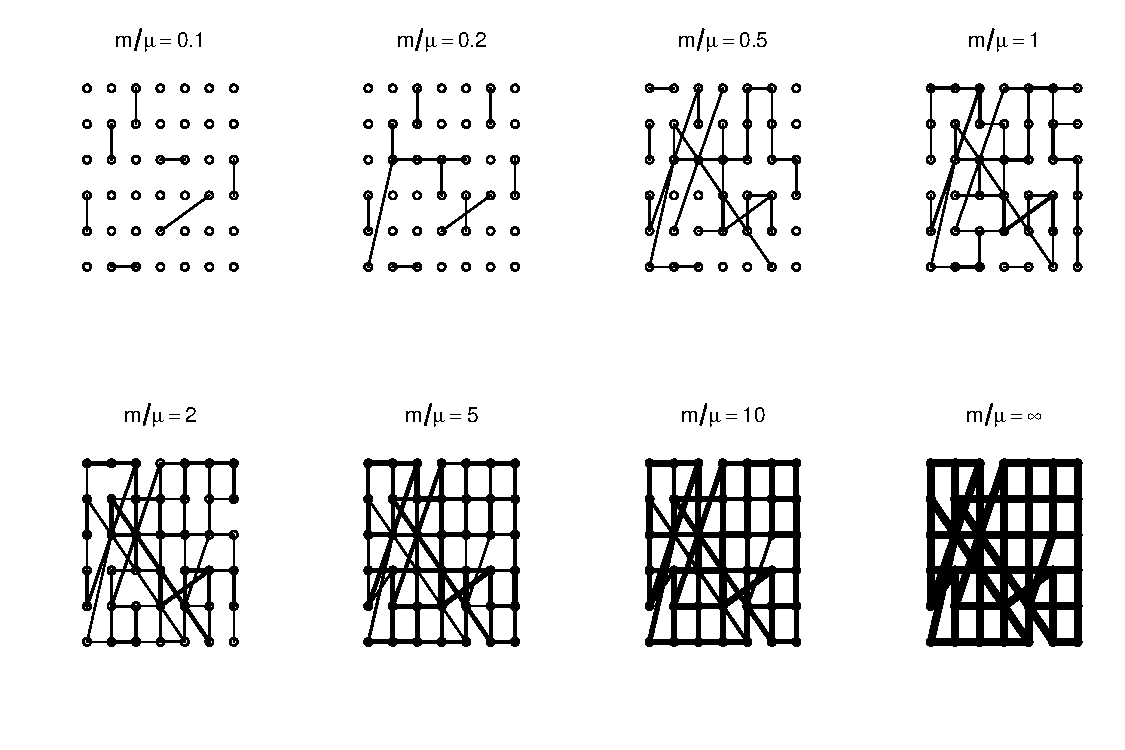
\includegraphics[scale=0.55]{plots/sample-graphs}}
  \end{center}
  \vspace{-2.5em}

  As $m / \mu$ increases, the sample Laplacian $L$ approaches the
  population Laplacian $\mathcal{L}$.
\end{frame}

\begin{frame}
  \begin{block}{Estimation performance}
    \begin{itemize}
      \item $\mathcal{\hat L}$ unregularized estimate, equal to observed Laplacian, $L$
      \item $\mathcal{\hat L}_\eta$ regularized estimate, gotten from solving (implicitly!) the
        Mahoney-Orecchia regularized SDP with $G(X) = -\log |X|$
      \item $\tau = \Tr(\mathcal{L}^+)$, $\Theta = \tau^{-1} \mathcal{L}^+$
      \item $\hat \tau = \Tr(\mathcal{\hat L}^+)$, $\hat \Theta = \hat \tau^{-1} \mathcal{\hat L}^+$
      \item $\hat \tau_\eta = \Tr(\mathcal{\hat L_\eta}^+)$, $\hat \Theta_\eta = \hat \tau_\eta^{-1} \mathcal{\hat L_\eta}^+$
      \item performance criterion is relative Frobenius error:
        \[
	  \|\Theta - \hat \Theta_\eta\|_\mathrm{F} / \|\Theta - \hat \Theta \|_\mathrm{F}
	\]
	where $\|A\|_\mathrm{F} = [\Tr(A' A)]^{1/2}$
      \item $\bar \tau$ is mean of $\tau$ over all replicates
      \item $\eta^\ast$ is optimal value of $\eta$
    \end{itemize}
  \end{block}
\end{frame}

\begin{frame}
	\centering
	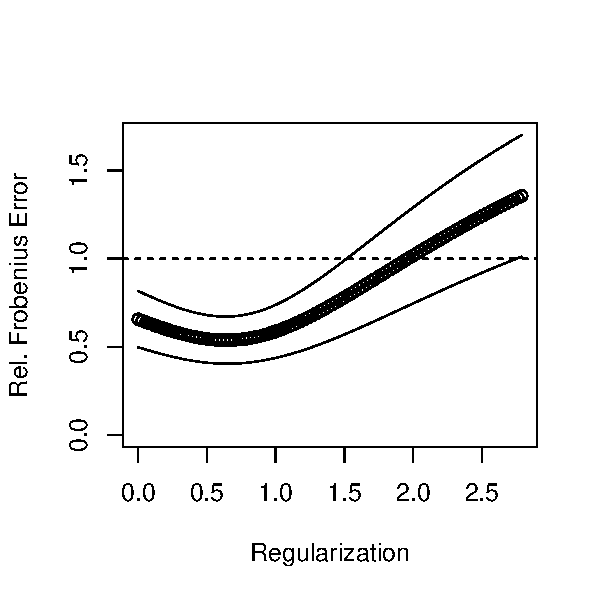
\includegraphics[scale=0.5]{plots/estimation-frob-p100}

	For certain values of $\eta$, the regularized estimate
	$\mathcal{\hat L}_\eta$ outperforms the unregularized
	estimate $\mathcal{\hat L}$, i.e.
	$\|\Theta - \hat \Theta_\eta\|_\mathrm{F}
	   / \|\Theta - \hat \Theta\|_\mathrm{F} < 1$.
\end{frame}

\begin{frame}
  \begin{center}
\begin{figure}[h]
  \subfigure{%[$m/\mu = 0.2$; $s = 0$.]{
    \makebox{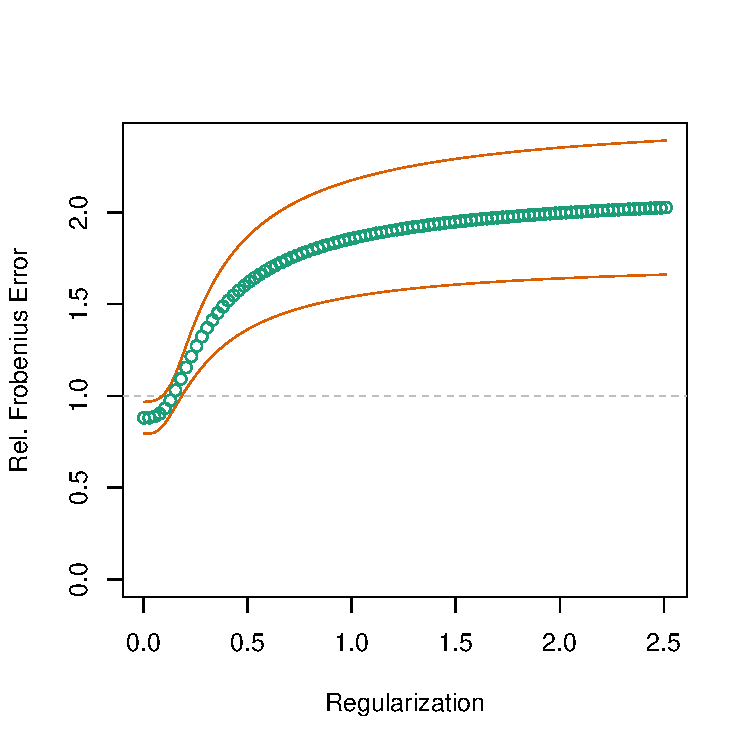
\includegraphics[scale=0.24]{plots/estimation-frob-s0-p020}}
  }
  \subfigure{%[$m/\mu = 1.0$; $s = 0$.]{
    \makebox{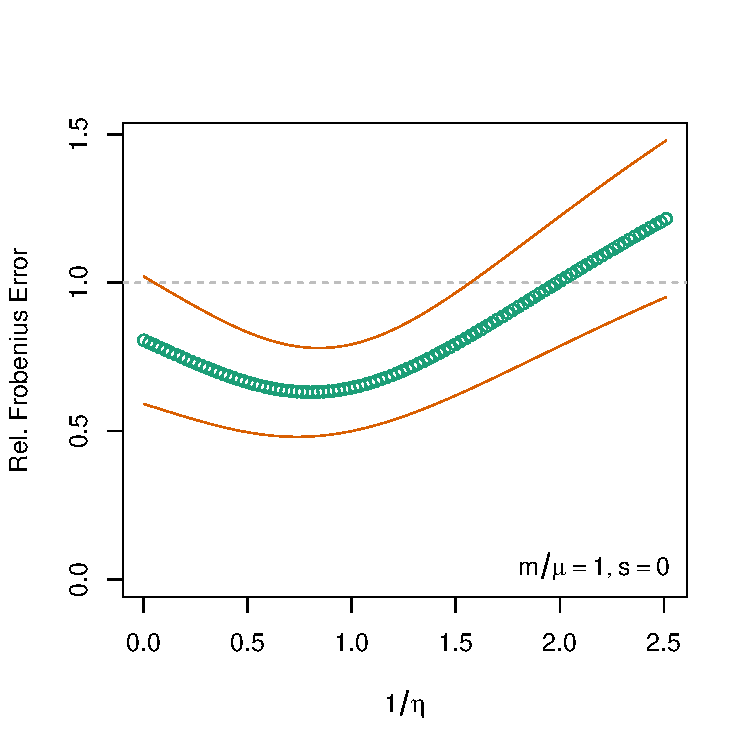
\includegraphics[scale=0.24]{plots/estimation-frob-s0-p100}}
  }
  \subfigure{%[$m/\mu = 2.0$; $s = 0$.]{
    \makebox{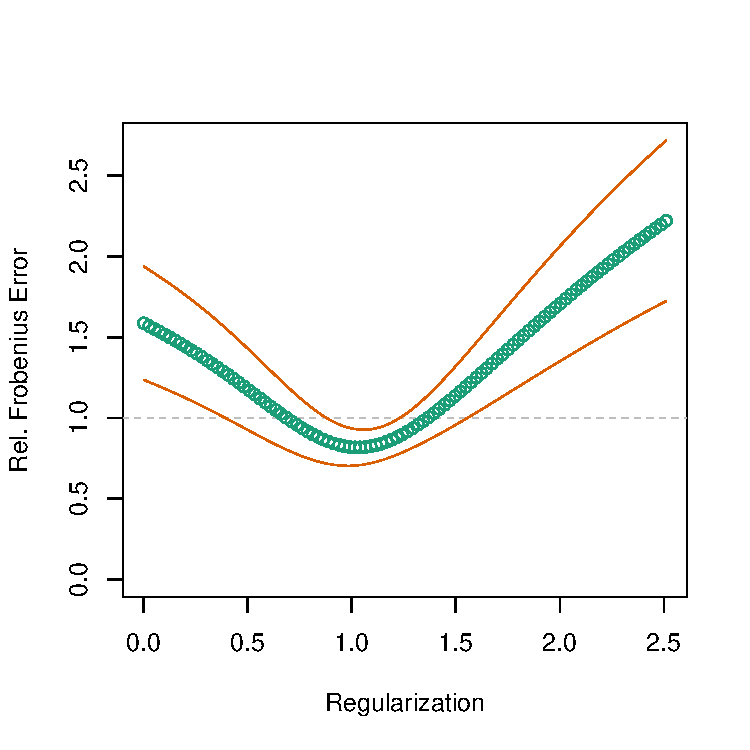
\includegraphics[scale=0.24]{plots/estimation-frob-s0-p200}}
  } \\
\vspace{-2.0em}
  \subfigure{%[$m/\mu = 0.2$; $s = 4$.]{
    \makebox{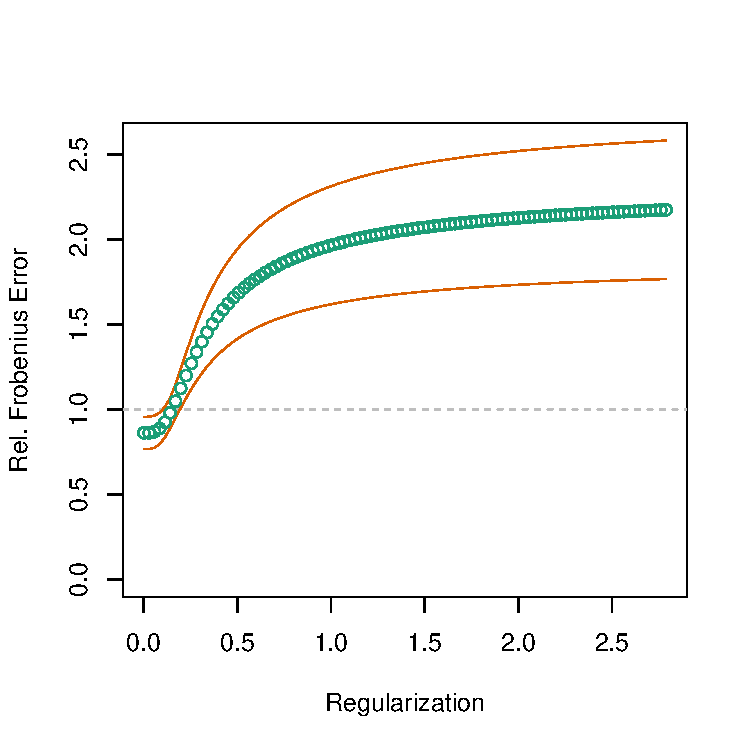
\includegraphics[scale=0.24]{plots/estimation-frob-p020}}
  }
  \subfigure{%[$m/\mu = 1.0$; $s = 4$.]{
    \makebox{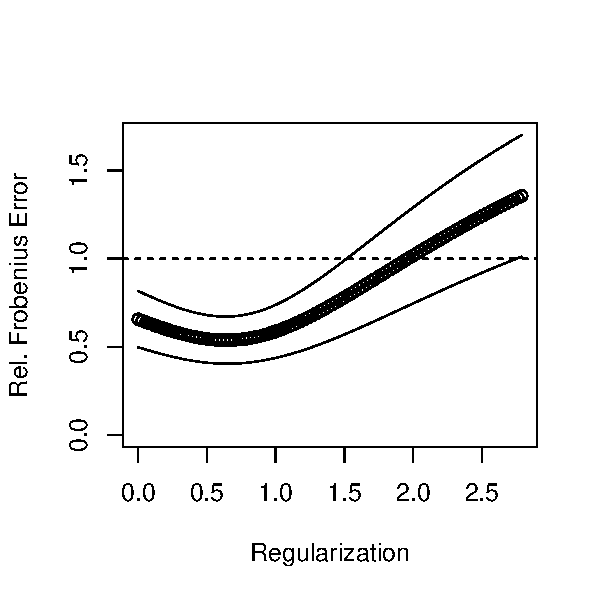
\includegraphics[scale=0.24]{plots/estimation-frob-p100}}
  }
  \subfigure{%[$m/\mu = 2.0$; $s = 4$.]{
    \makebox{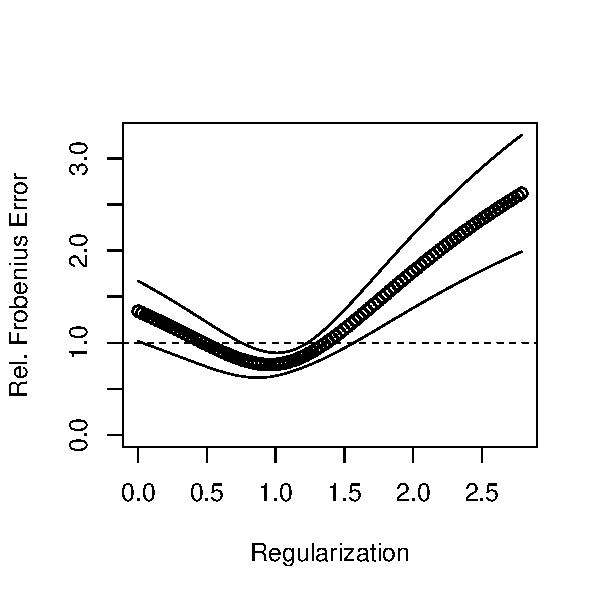
\includegraphics[scale=0.24]{plots/estimation-frob-p200}}
  } \\
\vspace{-2.0em}
  \subfigure{%[$m/\mu = 0.2$; $s = 32$.]{
    \makebox{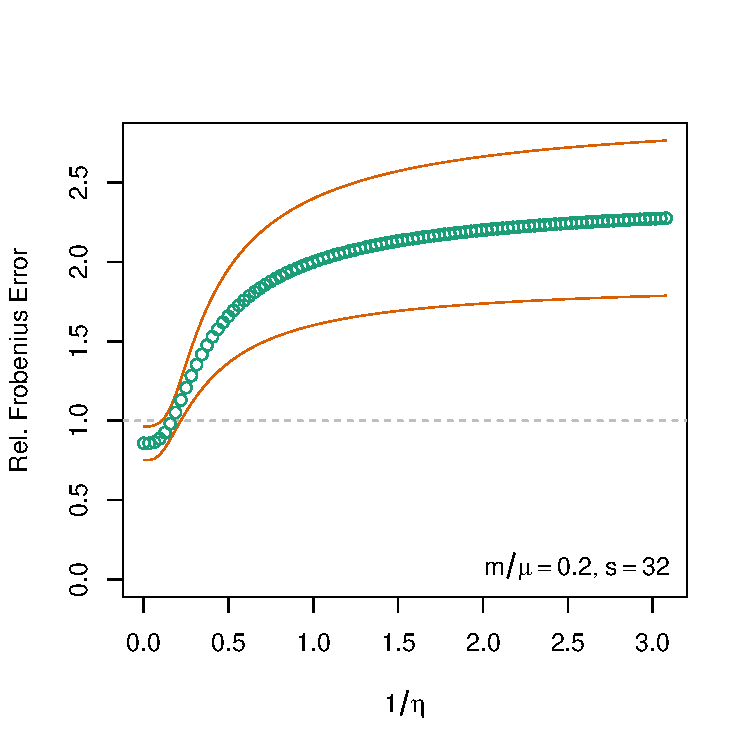
\includegraphics[scale=0.24]{plots/estimation-frob-s32-p020}}
  }
  \subfigure{%[$m/\mu = 1.0$; $s = 32$.]{
    \makebox{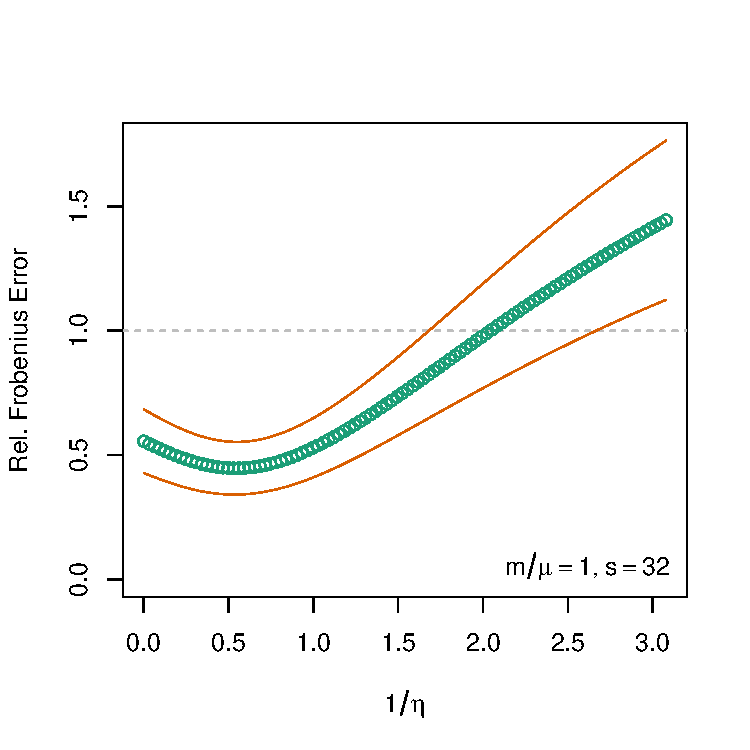
\includegraphics[scale=0.24]{plots/estimation-frob-s32-p100}}
  }
  \subfigure{%[$m/\mu = 2.0$; $s = 32$.]{
    \makebox{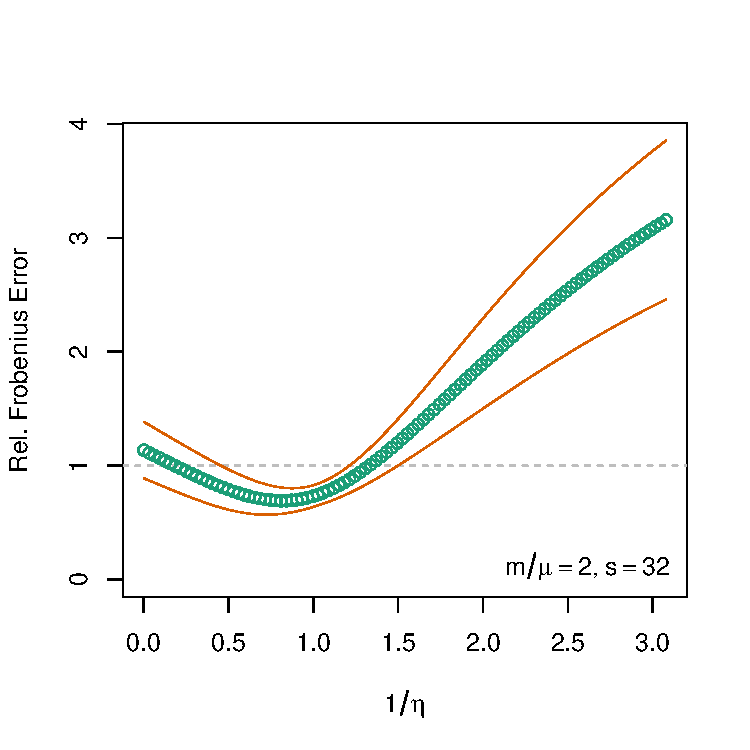
\includegraphics[scale=0.24]{plots/estimation-frob-s32-p200}}
  }
\setcounter{subfigure}{0}
\vspace{-2.5em}
\end{figure}
  \end{center}
The optimal regularization parameter $\eta^\ast$ depends on $m/\mu$ and
$s$.
\end{frame}

\begin{frame}
    \begin{center}
    \makebox{\label{F:optimal-frob}
             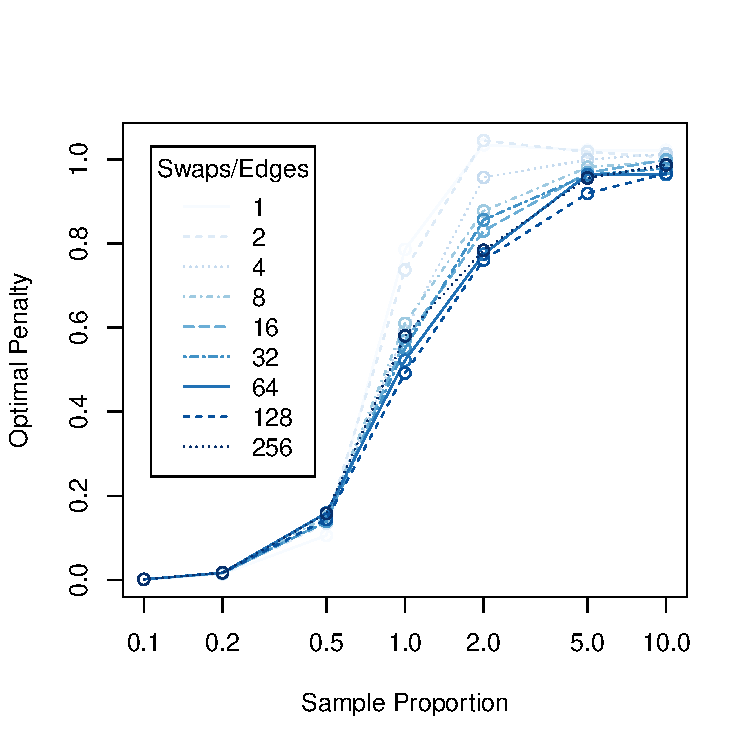
\includegraphics[scale=0.6]{plots/optimal}}
    \vspace{-2em}
  \end{center}
This figure plots the optimal regularization parameter 
$\eta^\ast / \bar \tau$ as a function of sample proportion for different
fractions of edge swaps.
\end{frame}

\begin{frame}
  \frametitle{References}
  \bibliographystyle{unsrt}
  \footnotesize{
    \bibliography{refs}
  }
\end{frame}

\end{document}
